%!TEX output_directory = aux

\documentclass[11pt]{article}

\usepackage[english]{babel}

% ---- FONT & MICROTYPOGRAPHY ----
\usepackage[utf8]{inputenc}
\usepackage[T1]{fontenc}
\usepackage{microtype}
\usepackage{moresize}

% ---- FORMATTING ----
\usepackage{csquotes,textcase,xspace}

% ---- PAGE LAYOUT ----
\usepackage{geometry}
\geometry{top=2.5cm,bottom=2cm,inner=2cm,outer=2cm,footnotesep=7mm plus 4pt minus 4pt}
\usepackage{setspace}
\setstretch{1.1}

% ---- GRAPHIQUE ----
\usepackage{graphicx}
\usepackage{xcolor}
\usepackage[font=small,labelfont=bf,labelsep=space]{caption}
\usepackage{subfigure}
\captionsetup{width=0.9\textwidth,font={small,stretch=1.1}}
\addto\captionsenglish{\renewcommand{\figurename}{Fig.}}
\addto\captionsenglish{\renewcommand{\tablename}{Tab.}}
\definecolor{JoliBleu}{rgb}{0,0.55,0.55}
\definecolor{JoliVert}{rgb}{0.15,0.6,0}
\definecolor{JoliRouge}{rgb}{0.86,0.08,0}
\definecolor{JoliJaune}{rgb}{1,0.75,0}
\definecolor{JoliGris}{rgb}{0.52,0.52,0.51}
\definecolor{myblue}{RGB}{26, 77, 116}
\definecolor{myorange}{RGB}{181, 116, 30}
\definecolor{mydarkorange}{RGB}{166, 88, 0}
\definecolor{mygreen}{RGB}{21, 124, 80}
\definecolor{myblack}{RGB}{43, 65, 82}
\definecolor{myred}{rgb}{0.5, 0.0, 0.13}

% ---- SECTIONING ----
\usepackage{titlesec}
\titleformat{\section}[block]{\Large\boldmath\bfseries}{\thesection}{1em}{}
\titleformat{\subsection}[block]{\large\boldmath\bfseries}{\thesubsection}{0.5em}{}
\usepackage{appendix}
\renewcommand{\setthesection}{\Alph{section}}
\renewcommand{\restoreapp}{}
\makeatletter
\renewcommand{\theequation}{\thesection.\arabic{equation}}
\@addtoreset{equation}{section}
\makeatother

% ---- FOOTERS HEADERS ----
\usepackage[bottom]{footmisc}
\usepackage{fancyhdr}

% ---- TABLE OF CONTENTS ----
\usepackage{titletoc}
\setcounter{tocdepth}{3}

% ---- BIBLIOGRAPHY ----
\usepackage[nosort]{cite}
\bibliographystyle{JHEP}
\newcommand{\eprint}[1]{{\href{http://arxiv.org/abs/#1}{\texttt{[#1]}}}}
\newcommand{\eprintN}[1]{{\href{http://arxiv.org/abs/#1}{\texttt{#1 [hep-th]}}}}
\newcommand{\doi}[2]{\href{http://dx.doi.org/#2}{#1}}

% ---- HYPER REF ----
\usepackage{hyperref}
\hypersetup{colorlinks=true,
        pdfstartview=FitV,
        linkcolor= mydarkorange,
        citecolor= mydarkorange, 
        urlcolor= JoliGris!60!black,
        hypertexnames=false,
        linktoc=page}

% ---- TIKZ ----
\usepackage{tikz}
\usetikzlibrary{calc}

% ---- MATHS ----
\usepackage{amsmath,amssymb,amsfonts,dsfont}
\usepackage{mathrsfs}
\usepackage{physics}
\usepackage{ytableau}
\ytableausetup{boxsize=1.1em,centertableaux}
\usepackage{stmaryrd}
\usepackage{nicefrac}
\allowdisplaybreaks[1]
% \usepackage{bbold}
\usepackage{cases}
\usepackage{bm}
\usepackage{bbm}

% ---- TABLES ----
\usepackage{multirow}
\usepackage{booktabs}
\usepackage{pdflscape}
\usepackage{array}
\usepackage{arydshln}

% ---- ENUMERATION ----
\usepackage[shortlabels]{enumitem}

% ---- MATHS COMMANDS ----
\newcommand{\A}{\ensuremath{\mathcal{A}}\xspace}
\newcommand{\F}{\ensuremath{\mathcal{F}}\xspace}
\renewcommand{\H}{\ensuremath{\mathcal{H}}\xspace}
\newcommand{\M}{\ensuremath{\mathcal{M}}\xspace}
\renewcommand{\P}{\ensuremath{\mathcal{P}}\xspace}
\newcommand{\J}{\ensuremath{\mathcal{J}}\xspace}
\renewcommand{\d}{\ensuremath{\mathrm{d}}\xspace}
\renewcommand{\H}{\ensuremath{\mathcal{H}}\xspace}
\newcommand{\SO}{\ensuremath{\mathrm{SO}}\xspace}
\renewcommand{\O}{\ensuremath{\mathrm{O}}\xspace}
\newcommand{\SL}{\ensuremath{\mathrm{SL}}\xspace}
\newcommand{\Odd}{\ensuremath{\mathrm{O}(d,d)}\xspace}
\newcommand{\odd}{\ensuremath{\mathfrak{o}(d,d)}\xspace}
\renewcommand{\Tr}[1]{\ensuremath{\mathrm{Tr}\left(#1\right)}\xspace}
\newcommand{\vol}{{\,\rm vol}}
\def\sst#1{{\scriptscriptstyle #1}}


\def\0{{\sst{(0)}}}
\def\1{{\sst{(1)}}}
\def\2{{\sst{(2)}}}
\def\3{{\sst{(3)}}}
\def\4{{\sst{(4)}}}
\def\5{{\sst{(5)}}}
\def\6{{\sst{(6)}}}
\def\7{{\sst{(7)}}}
\def\8{{\sst{(8)}}}

\newcommand{\be}{\begin{equation}}
\newcommand{\ee}{\end{equation}}

% ---- COMMENTS ----
\newcommand{\ce}[1]{\marginpar{\parbox{\marginparwidth}{\boldmath $\Longleftarrow$}}{\boldmath\bfseries (ce: #1)}}
\newcommand{\gl}[1]{\marginpar{\parbox{\marginparwidth}{\boldmath $\Longleftarrow$}}{\boldmath\bfseries (gl: #1)}}




%%%%%%%%%%%%%%%%%%%%%%%%%%%%%%%%%%
%%%%%%%%%%%%%%%%%%%%%%%%%%%%%%%%%%


\begin{document}

\begin{titlepage}



\begin{flushright}

MI-HET-??? \\
\today
\end{flushright}


\vspace{25pt}

   
   \begin{center}
   \baselineskip=16pt


   \begin{Large}

\mbox{ \bfseries \boldmath  Notes: Machine learning flat directions}
   \end{Large}


   		
\vspace{25pt}
		

{\large  Bastien Duboeuf$^{1}$, Camille Eloy$^{1}$ \,and\, Gabriel Larios$^{2}$}
		
\vspace{25pt}
		
		
	\begin{small}

	{\it $^{1}$ ENS de Lyon, CNRS, LPENSL, UMR5672,\\ 69342, Lyon cedex 07, France}  \\


	\vspace{10pt}
	
	{\it $^{2}$ Mitchell Institute for Fundamental Physics and Astronomy, \\
	Texas A\&M University, College Station, TX, 77843, USA}     \\
		
	\end{small}
		

\vskip 50pt

\end{center}


\begin{center}
\textbf{Abstract}
\end{center}


\begin{quote}

...

\end{quote}

\vfill

\end{titlepage}


\tableofcontents



\section{Introduction}

\section{Supergravity setup}
\begin{itemize}[label=\textbullet]
	\item Context: 6d ${\rm AdS}_{3}\times S^{3}$, truncation to 3d, potential, conformal manifold.
	\item Choice of truncation from 32 to 13 to 5 variables.
\end{itemize}

\paragraph{Potential}
The 22 scalars of the theory can be parametrised by ($22 = 32 - 10$, with 10 scalars gauge fixed using translations in the gauge group)
\begin{itemize}[label=\textbullet]
	\item $m = \nu\nu^{T}\in{\rm GL}(3,\mathbb{R})$ parametrizing the coset ${\rm GL}(3,\mathbb{R})/{\rm SO}(3)$,
	\item $\phi$ a $3\times3$ antisymmetric matrix,
	\item $\xi$ a $3\times4$ matrix, and $\xi^{2} = \xi \xi^{T}$,
	\item a dilaton $\tilde{\varphi}$.
\end{itemize}
We can further restrict ourselves to a set of 13 scalars (see ref.~\cite{Eloy:2021fhc}), with
\begin{equation}
	\begin{aligned}
		\xi &= \begin{pmatrix}
					0 & 0 & 0 & x_{1} \\
					0 & 0 & 0 & x_{2} \\
					0 & 0 & 0 & x_{3}
				\end{pmatrix},
		\quad
		\phi = \begin{pmatrix}
					0 & x_{4} & x_{5} \\
					-x_{4} & 0 & x_{6} \\
					-x_{5} & -x_{6} & 0
				\end{pmatrix},
		\quad
		\tilde{\varphi} = x_{13} \\[5pt]
		\nu &= e^{(6\,x_{7}+3\,x_{8}+\sqrt{3}\,x_{9})/6}
				\begin{pmatrix}
					1 & \frac{x_{10}}{\sqrt{2}} & \frac{x_{11}}{\sqrt{2}} + \frac{x_{10}x_{12}}{4} \\
					0 & e^{-x_{8}} & \frac{e^{-x_{8}}\,x_{12}}{\sqrt{2}} \\
					0 & 0 & e^{-(x_{8}+\sqrt{3}\,x_{9})/2}
				\end{pmatrix}.
	\end{aligned}
\end{equation}
Scalar potential from ref.~\cite{Eloy:2021fhc}:
%
\begin{equation} \label{eq:scalarpotential}
	\begin{aligned}
 		V & = 4\,e^{-4\tilde\varphi}+2\,e^{-2\tilde\varphi}\Big[-\tr\left(m+m^{-1}\right)+\tr\left(\phi m^{-1}\phi\right) -2\,\tr\left(\phi m^{-1}\xi^{2}\right)-2\,\tr\left(\xi^{2}\right)\\
 		&\qquad\quad-\tr\left(\xi^{2}m^{-1}\xi^{2}\right)  +\frac{1}{2}\,\det\left(m^{-1}\right)\left(1-\tr\left(\phi^{2}\right)-\tr\left(\xi^{4}\right)+\tr\left(\xi^{2}\right)^{2}\right) \\
 		&\qquad\quad +\frac{1}{2}\,{\rm T}\left(m^{-1}(\xi^{2}-\phi),(\xi^{2}+\phi)m^{-1},m+(\xi^{2}+\phi)m^{-1}(\xi^{2}-\phi)+2\,\xi^{2}\right)\\
 		&\qquad\quad +\frac{1}{4}\,{\rm T}\left(m^{-1},m+(\xi^{2}+\phi)m^{-1}(\xi^{2}-\phi)+2\,\xi^{2},m+(\xi^{2}+\phi)m^{-1}(\xi^{2}-\phi)+2\,\xi^{2}\right)\Big], 
 	\end{aligned}
\end{equation}
where ${\rm T}\left(A,B,C\right)=\varepsilon_{mnp}\,\varepsilon_{qrs}\,A^{mq}B^{nr}C^{ps}$.

As a first simplified example we have considered only the parameters $x_{1}, x_{2}, x_{4}, x_{8}$ and $x_{10}$. The potential~\eqref{eq:scalarpotential} becomes
\begin{equation} \label{eq:scalarpotential124810}
	\begin{aligned}
		V &= \frac{1}{8}\, e^{-2\,x_{8}} \bigg[4 + 4\,x_{1}^4 + e^{4\,x_{8}} \big(2 + x_{10}^2\big)^2 \big(1 + x_{2}^4\big)\\
		  & \quad\qquad\qquad - 4\,e^{3\,x_{8}}\,\big(2 + x_{10}^2\big) \Big(2 - x_{1}^2 + \sqrt{2}\,x_{1} x_{10} x_{2}^3 + x_{2}^4 + 
      			2\,x_{1} x_{2} x_{4} + x_{4}^2 - x_{2}^2 \big(1 - x_{1}^2 + x_{4}^2\big)\Big)\\
        & \quad\qquad\qquad - 8\,e^{x_{8}}\,\Big(2 + x_{1}^4 + \sqrt{2}\,x_{1}^3 x_{10} x_{2} - x_{2}^2 - 2\,x_{1} x_{2} x_{4} + 
      			x_{4}^2 - x_{1}^2 \big(1 - x_{2}^2 + x_{4}^2\big)\Big)\\
        & \quad\qquad\qquad + 4\,e^{2\,x_{8}}\,\Big(2 - 4\,x_{1}^2 + x_{1}^4 - 4\,x_{2}^2 + 4\,x_{1}^2 x_{2}^2 + x_{2}^4
        			+ x_{10}^2\big(1 + 3\,x_{1}^2 x_{2}^2\big) + 4\,x_{4}^2 + x_{4}^4\Big)\\
        & \quad\qquad\qquad + 8\sqrt{2}\,x_{10}\,e^{2\,x_{8}}\,\Big(x_{1}^3 x_{2} + x_{1}^2 x_{4} - x_{2}^2 x_{4} + x_{1} \big(x_{2}^3 - x_{2} x_{4}^2\big)\Big)\bigg].
	\end{aligned}
\end{equation}
\ce{Change notation to keep $x$ for the polynomial variables?}

\ce{Discuss here why we need numerical methods: to complicated for mathematica to simplify the gradient.}

\section{Numerical analysis}
	\subsection{Gradient descent and local analysis}
		\paragraph{Gradient descent: implementation, sampling, time needed, loss}

		To identify the flat directions in the potential, we will use numerical tools. The procedure is as follows: first, we sample the underlying manifold, and then we use numerical techniques to extract analytical information from the resulting cloud of points. The first step is thus to sample the manifold.
		
		To do so, we perform a basic gradient descent. We begin by randomly and uniformly initializing points within a hypercube of range $[-2,2]$. This choice is important to ensure that points are not restricted to the inner range $[-1,1]$. For this example, we choose to generate $10^5$ points. This number is motivated by the dimensionality of our problem. If we aim to populate all possible directions and want approximately $\mathcal{O}(10)$ points per direction, then we require $\mathcal{O}(10^5)$ points. Given that the true intrinsic dimensionality of the manifold is less than or equal to 5, this value serves as a conservative upper bound for the number of points needed to adequately sample the manifold.
		
		We then perform gradient descent on the points using TensorFlow’s automatic differentiation. The loss function is defined as:
		\begin{equation}
			\mathcal{L} = \sum_{i = 1}^{n_{points}} || \nabla V(\vec{x}^{,i})||^2
		\end{equation}
		where $\vec{x}^{\,i} = (x^i_1,x^i_2,x^i_4,x^i_8,x^i_{10})$ denotes the data points. We use the Adam optimizer with a learning rate of $10^{-2}$ and run the gradient descent for $10,000$ epochs to ensure convergence.
		
		% \begin{figure}
			% \includegraphics[scale = 0.5]{imagefile} % add loss history
			% \end{figure}
		
		As a first visualization, we present a triangular plot of the data in Fig. \ref{triangular_plot_1_2_4_8_10}. This figure shows all possible 2D projections of the data, along with the 1D histograms of each coordinate after gradient descent.
		
		\begin{figure}[t]
			\centering
			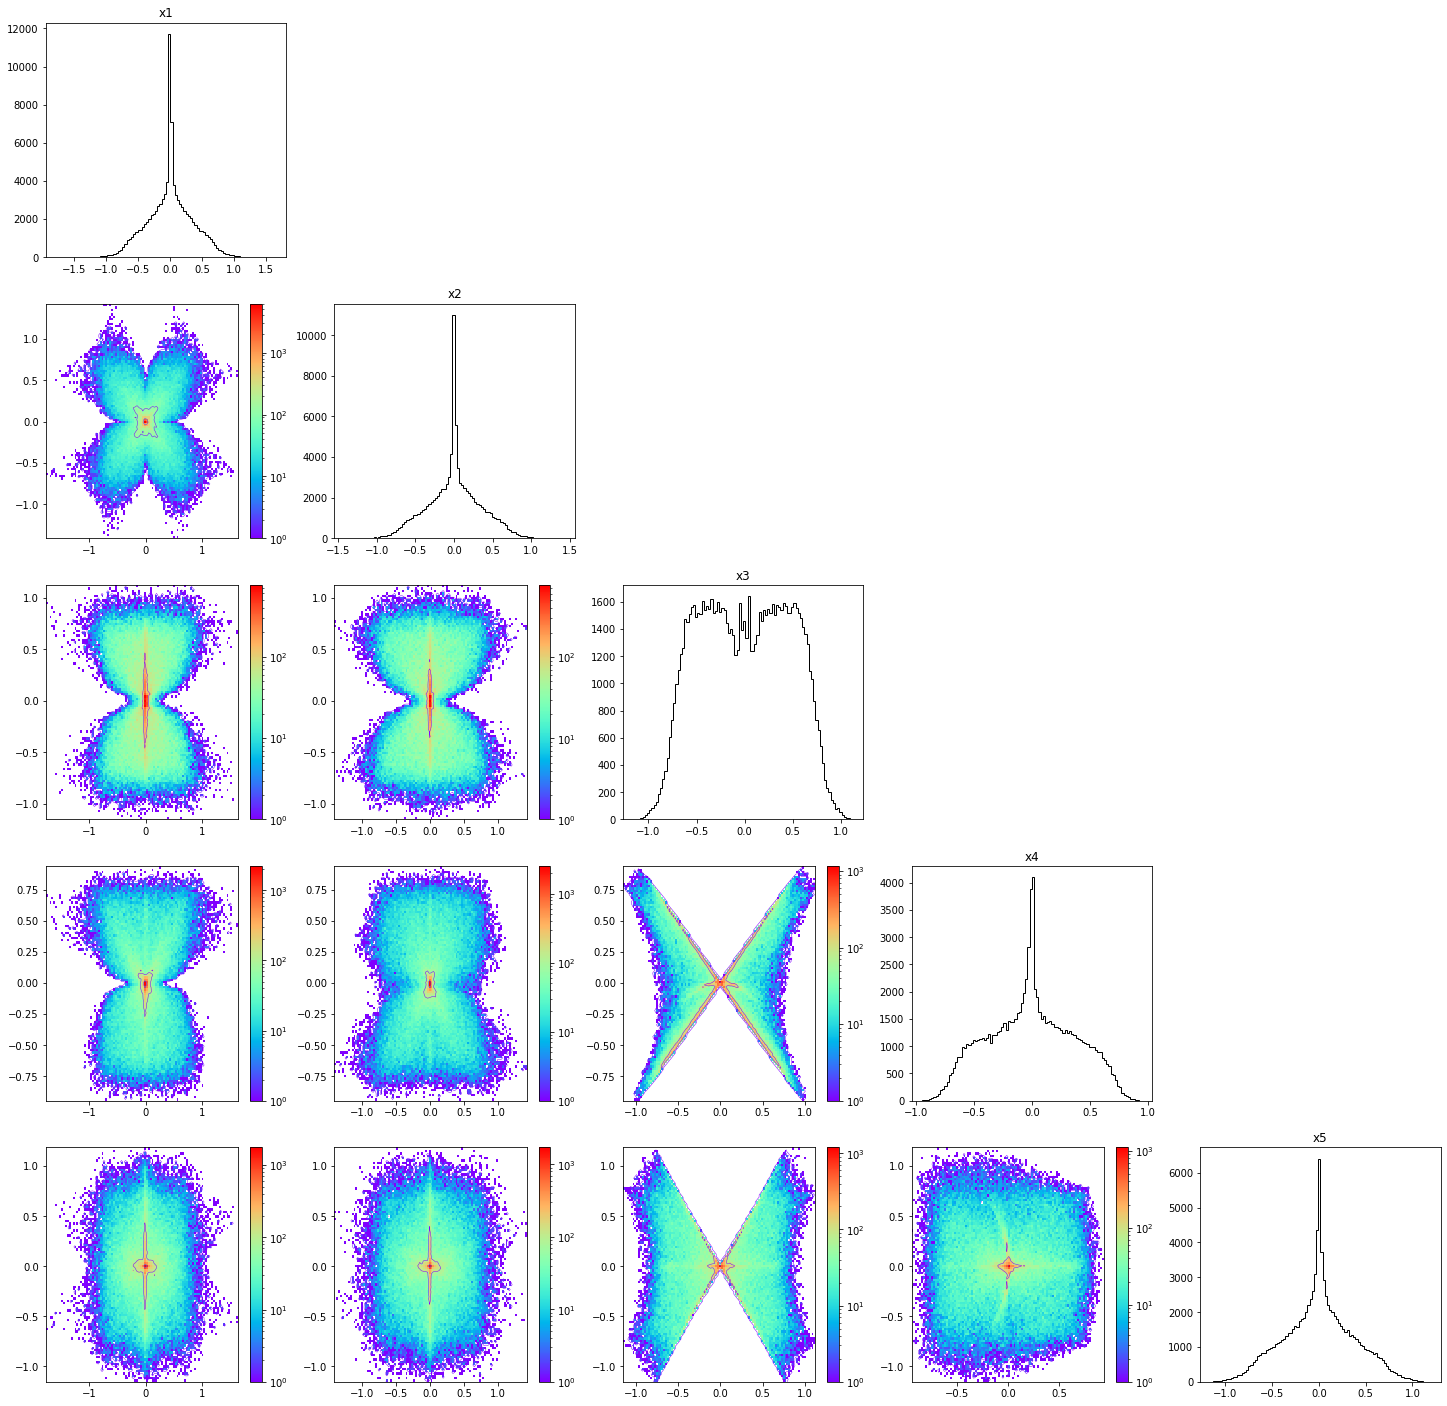
\includegraphics[scale = 0.25]{Figures/triangular_plot_1_2_4_8_10.png} %names need to be changed.
			\caption{Triangular plot showing $2d$ projections and $1d$ histograms of the data after the gradient descent}
			\label{triangular_plot_1_2_4_8_10}
		\end{figure}
		
		We can make a few comments on those plots. First, we observe non-trivial correlations in the data. Some of these may result from larger basins of attraction, such as in the $x_1/x_2$ plot. However, the structures seen in the $x_4/x_8$ or $x_4/x_{10}$ plots likely reflect genuine features of the manifold, and will show latter that this is indeed the case. We also note that alll directions appear to be well populated. Furthermore, we can notice that a large majority of the points converge to the origin $\vec{0}$. This is not surprising, as this just mean that the round sphere solution has a larger basin of attraction, which sounds reasonable. We do not however attempt to shift the points along flat directions to depopulate the origin or repopulate other regions.

		\paragraph{Local PCA: graphs of number of patches with given local dimension, and with varying size of local patch, discuss optimal patch size (we want at least fex points in each direction)}

		Once the gradient descent has been completed and the flat direction sampled, the next step is to identify the structure of the underlying manifold. Our goal is to eventually obtain an analytical expression, not just a numerical description. Before applying symbolic regression to search for such an expression, we can first perform some exploratory analyses to better understand the data. Specifically, we aim to determine the dimensionality of the manifold and whether it consists of a single connected component or multiple disjoint components (e.g., two intersecting hyperplanes).
		
		To this end, we apply a local Principal Component Analysis (PCA). For each point, we identify its $k$ nearest neighbors and perform a PCA on that local neighborhood. This procedure allows us to determine how many principal directions are needed to explain a given proportion $\epsilon$ of the data variance. In other words, it provides an estimate of the local dimensionality around each point.
		
		We perform this analysis for several values of $k$, namely $k \in \{5, 10, 20, 50, 100\}$, and we fix $\epsilon = 0.99$. The results are presented in Fig. \ref{local_pca}.
		
		\begin{figure}
			\centering
			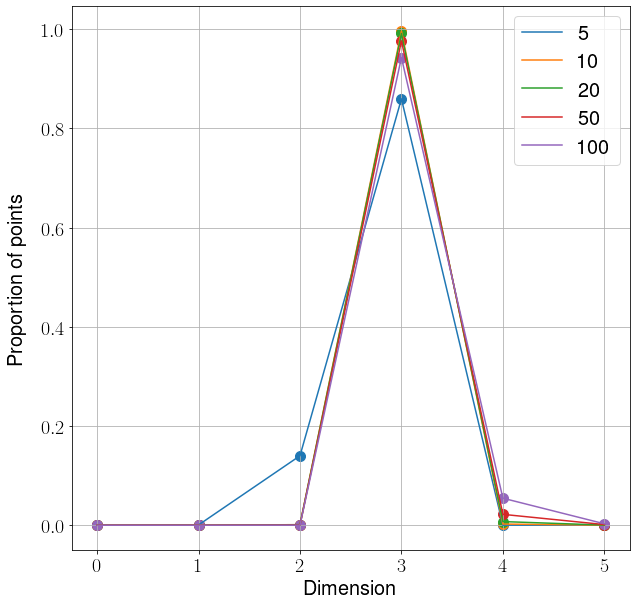
\includegraphics[scale=0.5]{Figures/Local_PCA.png}
			\caption{Results of the local PCA analysis. The $x$-axis shows the dimension inferred by the algorithm, and the $y$-axis indicates the proportion of points for which that dimension was found. Each curve corresponds to a different value of $k$ in the $k$-nearest neighbors.}
			\label{local_pca}
		\end{figure}
		
		We observe that for every choice of $k$, there is a prominent peak at $d = 3$, suggesting that the underlying manifold is three-dimensional. For $k = 5$, a noticeable fraction of points are assigned a dimensionality of 2. This can be attributed to the fact that if the true dimension is 3, then selecting only 5 neighbours may not sufficiently populate all three directions, leading the algorithm to underestimate the dimensionality.
		
		Additionally, for $k \geq 20$, we observe an increasing number of points being assigned dimensionalities of 4 or 5. This behavior can be explained by the loss of locality when the number of neighbours becomes too large: increasing $k$ results in a coarser approximation, and the algorithm may then incorporate points that are no longer truly local. This artificial enlargement of the neighborhood can cause the estimated local dimensionality to rise.
		
		We thus conclude that the manifold under investigation has an intrinsic dimension of 3.
		
		\paragraph{Clusteting: HDBScan (only parameter: minimal number of points in a cluster), and graphs of 3d slices of the 5d space}
		
		One possible scenario is that our data actually consists of several distinct three-dimensional manifolds, and the points previously identified with dimension $4$ may lie at the intersections of these manifolds. To illustrate, consider the intersection of two lines: at the intersection point, the local dimensionality estimated by the previous PCA algorithm would be 2. To rule out this possibility, we apply a clustering algorithm based on local density, where we only select the points of dimension 3. This, way, we remove the possible intersection points with dimension 4. For the purpose of the clustering, we use the HDBSCAN algorithm\footnote{Details of the algorithm can be found in the original HDBSCAN paper or documentation. Briefly, it is a density-based clustering method that extends DBSCAN by converting it into a hierarchical clustering algorithm and then extracting a flat clustering based on the stability of clusters.}.
		
		We set the minimum cluster size to 10 points. Out of the 986,060 3-dimensional points, the algorithm identifies three clusters: one of size 10, one of size 91,747, and one of size 6,849.
		
		The smallest cluster (10 points) is likely an artifact of local fluctuations in the data density and is not interpreted as physically meaningful. The last group, comprising 6,849 points, consists of points that the algorithm could not assign to any cluster. We interpret these as outliers or edge points rather than representatives of a separate manifold.
		
		What the algorithm does indicate, however, is that over 90\% of the data belongs to a single dominant cluster. In Fig.~\ref{3dplots}, we show 3D projections of the data to visualize the clustering.
		
		\begin{figure}
			\centering
			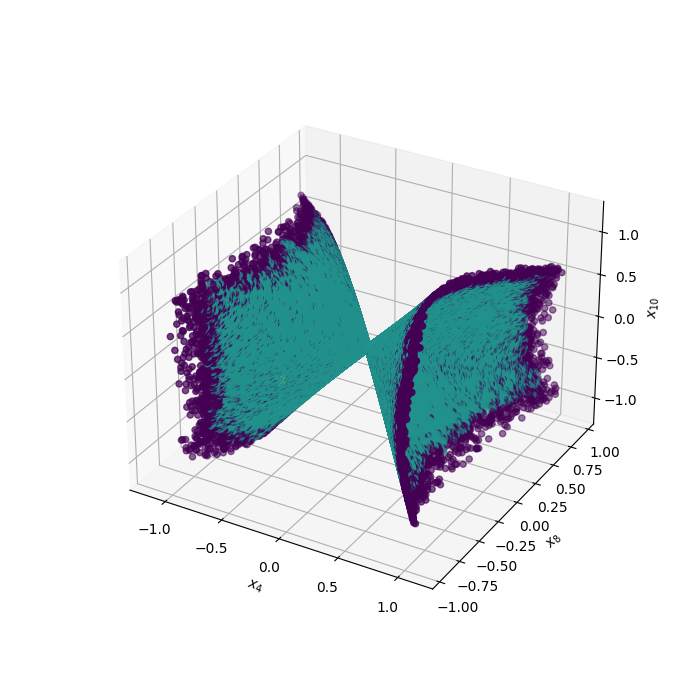
\includegraphics[scale=0.4]{Figures/3d_plot_x4_x8_x10.png}
			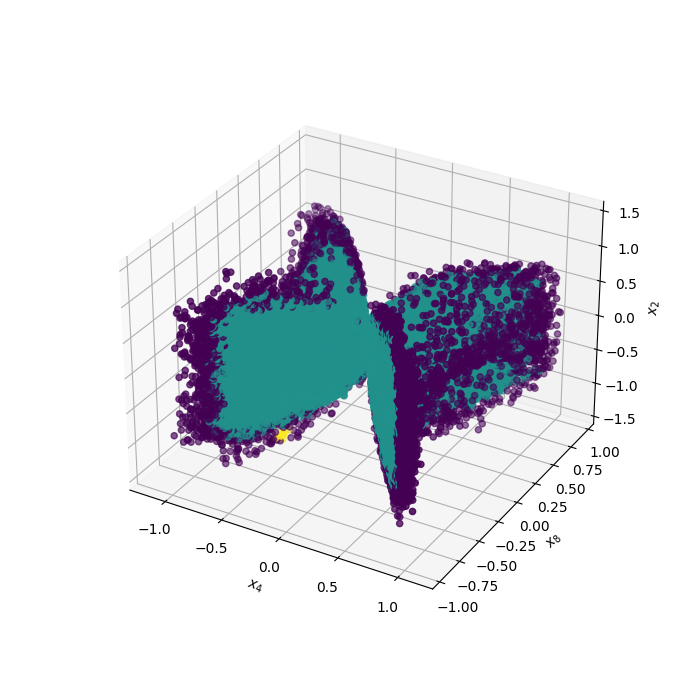
\includegraphics[scale=0.4]{Figures/3d_plot_x2_x4_x8.png}
			\caption{3D plots of the data in selected coordinates. Left: $(x_4, x_8, x_{10})$. Right: $(x_2, x_4, x_8)$.}
			\label{3dplots}
		\end{figure}
		
		In these scatter plots, turquoise points belong to the main cluster, while purple points are those that the algorithm failed to assign. In one of the plots, a few yellow points can be seen; these correspond to the smallest cluster of 10 points. From visual inspection, it appears that the unassigned (purple) points lie mostly on the boundary of the sampled region. We therefore interpret their unassigned status not as evidence of belonging to another manifold, but rather as a result of insufficient local density near the edges of the dataset.
		
		From this analysis, we conclude that the gradient descent procedure has produced a sampling of a single, connected, three-dimensional manifold.
		
		\vspace{0.5em}
		
		After performing both PCA and clustering, we thus confirm that the data obtained after gradient descent samples a three-dimensional manifold.

	\subsection{Annealed Importance Sampling for polynomial symbolic regression}
	\begin{itemize}[label=\textbullet]
		\item We can convert the potential to a polynomial by converting the variables that appear in exponentials to logs.
		\item As the potential is a polynomial, the solutions satisfy polynomials equations. Discuss that fact that we could get polynomials directly by taking the gradient of the potential, but those will be to complicated to express the vacuum in a usable way.  We search those using Annealed Importance Sampling.
		
		Now we have sampled the manifold and exctrated some basic information about it (namely its dimension and the fact that it is made of one block), we would like to see if we can exctract some analytic formula to caracterise it. What we have at the moment, are points on a 3-dimensional manifold, which are embedded in a 5-dimensional space. Therefore we can conclude that, in order to caracterise the manifold, we need two constraints on the embedding coordinates $\vec{x} = (x_1,x_2,x_4,x_8,x_{10})$. If we have a look at the form of the potential \eqref{eq:scalarpotential124810}, we see that if we use $\tilde{x_{8}} = e^{x_8}$, that this potential is actually a polynomial of the embedding coordinates. Therefore, the components of $|\nabla V|$ are also polynomials in those variables. We conclude that the constraints on the embedding coordinates we are looking for are polynomial constraints of the form $p(\vec{x}) = 0$, and that there are two of those. Of course if one takes directly the gradient of \eqref{eq:scalarpotential124810}, one ends up with such conditions, but none are usable directly to solve for two of the variables in terms of the others. The problem we are facing here is therefore a problem of symbolic regression : we are looking for analytic expressions (polynomial) that vanish once evaluated on our data points. There are a number of way one can deal with it, using already existing methods such as AI Feynman methods, or ..., or by doing rough gradient descent on the most general polynomial with arbitrary coefficients and trying to minimize its value once evaluated on the data points. In the spirit of trying to build a generalisable method, we develop here our own method, which is based on symbolic regression using an Annealing Importance Sampling method. 

		\item Annealed Importance Sampling: first explain general idea (construct density probability, role of temperature, links with Monte-Carlo), discuss $\beta$ to control exploration and exploitation phases.
		
		In the realm of symbolic regression, the objective is to uncover interpretable mathematical expressions that best describe a given dataset. In the problem discussed in this paper, we are looking for polynomial expressions such that $p(data) = 0$. This task involves navigating a vast, discrete, and often rugged search space of possible symbolic models, which poses significant challenges for traditional sampling methods. Markov Chain Monte Carlo (MCMC) techniques, while widely used, can struggle with poor mixing and getting trapped in local optima, especially in high-dimensional or multimodal spaces.
		
		To address these challenges, we employ an Annealed Importance Sampling (AIS) combined with Sequential Monte Carlo (SMC) methods. AIS constructs a sequence of intermediate distributions that smoothly transition from an initial, tractable distribution (e.g., a prior over symbolic expressions) to the complex target posterior distribution. This annealing process is guided by a temperature-like parameter that gradually emphasizes the data likelihood, allowing for more efficient exploration of the probability landscape.
		
		SMC enhances this procedure by propagating a population of particles—each representing a candidate symbolic expression—through the sequence of distributions. At each step, particles are reweighted based on the incremental change in the distribution, resampled to focus computational effort on high-probability regions, and mutated via operations. This combination of importance sampling, resampling, and mutation maintains diversity among the particles and prevents premature convergence to suboptimal models.
		
		These features make AIS-SMC particularly well-suited for symbolic regression tasks, where the search space is not only high-dimensional but also structured and discontinuous. 
		
		\item Then more details: discuss hypotheses to compute the weights, choice of transformations, choice of $\beta$, choice of loss, prior, initial sampling, choice of representation for the polynomials.
		
		Let us now explain in more details how does this procedure goes. The goal is to reconstruct some distribution function $p(z)$, where here $z$ in going to be some polynomial. We will try to reconstruct this density function by a serie of density function $\pi_n(z_n) = \gamma_n(z_n)/Z_n$ with $n = 1,\dots,N$ is going to be the number of annealing steps, $\pi_n$ is defined in terms of an unnormalized density $\gamma_n$ and we have the normalizing constant $Z_n = \int \gamma_n(z) \mathrm{dz}$. We also assume we have a sequence of inverse temperature constants $\beta_n$, where $0 = \beta_1 < \beta_2 <\dots< \beta_N = 1$. We then define the unnormalized density at level $n$ in terms of a prior distribution $p_0(z)$ over the hypothesis space and an Loss function $L(z)$
		\begin{equation}
			\gamma_n(z) := p_0(z) \: \exp \left( -\beta_n L(z) \right)
		\end{equation} 
		
		At each step, we have a set of particles $\{z_{n-1}^k, w_{n-1}^k\}$ approximating $\pi_{n-1}$ (meaning $\mathbb{E}_{\pi_{n-1}}[f] \approx \frac{\sum_k w_{n-1}^k f(z_{n-1}^k)}{\sum_k w_{n-1}^k}$), and we want to obtain a new set $\{z_n^k, w_n^k\}$ approximating $\pi_n$. To do so, for each particle $z^k_{n-1}$, we propose a new particle $z_n^k \sim q(z_n | z_{n-1}^k)$ and walculate the new unnormalized importance weight $w_n^k$. The latter are updated using the formula 
		\begin{equation}
			w_n^k = w_{n-1}^k \times \alpha_{n}^k
		\end{equation}
		where $\alpha_n^k$ is the incremental importance weight. The standard form for $\alpha_n^k$, which requires introducing an auxiliary backward transition kernel $q(z_{n-1} | z_n)$, is:
		\begin{equation}
			\alpha_n^k = \frac{ \gamma_n(z_n^k) q(z_{n-1}^k | z_n^k) }{ \gamma_{n-1}(z_{n-1}^k) q(z_n^k | z_{n-1}^k) } 
		\end{equation}
		The weights are finally normalized and we get $w_n^k \rightarrow \frac{w_n^k}{\sum_j w_n^j}$.
		
		Let's us now focus on the forward ($q(z_n^k | z_{n-1}^k)$) and backward propagation kernel ($q(z_{n-1}^k | z_n^k)$). The forward propagation kernel defines how we generate the state at time $n$ given the state at time $n-1$. It gives the probability to transition from $z_{n-1}$ to $z_n$. The backward kernel: It represents a hypothetical probability of transitioning back from state $z_n$ to state $z_{n-1}$. The purpose of $q$ is to give a proposition for $z_n$ given $z_{n-1}$. For the implementation of the two, we decide to implement an AIS-style MCMC code : we make some move in the space of polynomials, and then accept or reject those new polynomials based on an acceptance rate. So we first need to choose what are the available moves in the space of polynomials. Here are the choices we have made for our symbolic regression task : 
		\begin{itemize}
			\item Coefficient pertubation. Given a polynomial $z_{n-1}$, we choose randomly one of his coefficient and modify it by a random noise from the guassian distribution $\mathcal{N}(0,\sigma^2)$. So for eg : $2 x + 3 y^2 \rightarrow  2.1 x + 3 y^2$.
			\item Variable multiplication. Given a polynomial $z_{n-1}$, we choose randomly one of his monomial, and multiply it by one of the available variable. So for eg : $2 x + 3 y^2 \rightarrow  2 x y + 3 y^2$.
			\item Variable division. Given a polynomial $z_{n-1}$, we choose randomly one of his monomial, and divide it by one of its variable. So for eg : $2 x + 3 y^2 \rightarrow  2 x y + 3 y^2$.
		\end{itemize}
		This implementation allows us to straightforwardly calculate the forward and backward propagation kernel.  For example, the case of the coefficient pertubation is symmetric. Therefore $q(z_n^k | z_{n-1}^k) = q(z_{n-1}^k | z_n^k)$, which allows to simplify the calculation of the incremental importance weight. 
		
		The acceptance ration for the MCMC algorithm is given by : 
		\begin{equation}
			A(z_n,z_{n-1}) = \mathrm{min} \left(1,\frac{ \gamma_n(z_n^k) q(z_{n-1}^k | z_n^k) }{ \gamma_{n-1}(z_{n-1}^k) q(z_n^k | z_{n-1}^k) }  \right)
		\end{equation}
		We then draw $u\sim \mathrm{Uniform}(0,1)$, accept the new particle if $u<A(z_n,z_{n-1})$ and reject it otherwise.
		
		Before closing the section, we need to discuss what is the Loss function we choose. It is recquired to compute the unormalized distribution $\gamma_n$. Assume that we have $z = \sum_k c_k X_k$, where $c_k$ are the coefficients of the polynomials, and $X_k$ is a short notations for all the possible monomials up to a given degree (so if we have $x$ and $y$ as variables, and the maximum degree is 2, then $X_k$ are $1, x, y, x^2, y^2, x y$). For the Loss function, we decided to take : 
		\begin{equation}
			L(z) = \sum_{i} z(x_i)^2 + \frac{\lambda}{\sum_k c_k}
		\end{equation}
		So the first term is just the sum of the squared of the polynomial evaluated on the data. We want to make this 0 so we find polynomial that annihilates our data. The second part is a regularisation factor : it prevents the algorithm to send all the coefficient to 0, which would give a trivial solution to the problem. We typically take $\lambda \sim \mathcal{O}(1000)$.

		\item Discuss the fact that we allow float coefficients even though we know the coefficients will be only integers of square roots of integers?
		
		\item Analysis after AIS: select the best polynomials and do exploitation on the coefficients (without MC: we keep only the proposal of it betters the polynomial).
		
		Once the Annealing loop is over, we end up with a total of $n_{sample}$ particles, which in principle should be close to annihilate our data, but whose coefficient may need some more fine tuning. To deal with it, we ran a quick exploitation phase, where, for each polynomial, we now only modify its coefficients, with a pertubation $\epsilon \sim \mathcal{N}(0, \sigma_1)$, and keep the new particle, only if the Loss function is now getting smaller. This allow to fine-tune the coefficients. 
		
		\item Results for naive choices of parameters (numbers of iteration and particles, probabilities, $\beta$) and motivate them (we want some exploration and then exploitation, not too long computations): for multiple runs we find multiple polynomials (good polynomial: after exploitation we convert the coefficients to integers and square roots, and recompute loss without regularisation, select with threshold). Quantify it nicely: success rates for each polynomials, and absolute number of success, failing rate. Total time needed, without cluster or fancy computers.
	\end{itemize}
	
	\paragraph{Results}
	We have used the numerical analysis outlined in the previous sections to the search for extrema of the scalar potential~\eqref{eq:scalarpotential124810}. The code finds the 7 different following polynomials: \ce{Mention that we ``rounded'' the coefficients to integer and square root of them.}
	\begin{subequations} \label{eq:pols}
    \begin{align}
      p_{1} &= -\sqrt{2}\,x_{1} + \sqrt{2}\,x_{1}\tilde{x}_{8} + x_{2}\tilde{x}_{8}x_{10} - \sqrt{2}\,x_{2}x_{4}\tilde{x}_{8},\\
      p_{2} &= 2\,x_{2} - 2\,x_{2}\tilde{x}_{8} + \sqrt{2}\,x_{1}x_{10} + 2\,x_{1}x_{4} - x_{2}\tilde{x}_{8}x_{10}^{2},\\
      p_{3} &= 2\,x_{2} - 2\,x_{2}\tilde{x}_{8} + \sqrt{2}\,x_{1}\tilde{x}_{8}x_{10} + 2\,x_{1}x_{4}\tilde{x}_{8}
      		- 2\,x_{2} x_{4}^{2}\tilde{x}_{8},\\
      p_{4} &= \sqrt{2}\,x_{2} - \sqrt{2}\,x_{2}\tilde{x}_{8} + \sqrt{2}\,x_{1}\,x_{4} + x_{1}\tilde{x}_{8}x_{10}
      		- x_{2}x_{4}\tilde{x}_{8}x_{10},\\
      p_{5} &= -2\,x_{1} - 2\,x_{2}x_{4}- 2\,x_{1}x_{4}^{2} + 2\,x_{1}\tilde{x}_{8} + \sqrt{2}\,x_{2}x_{10}
      		+ x_{1}\tilde{x}_{8}x_{10}^{2},\\
      p_{6} &= -2\,x_{2}x_{4} - 2\,x_{1}x_{4}^{2} + 2\,x_{2}x_{4}\tilde{x}_{8} + \sqrt{2}\,x_{2}x_{10} 
      		- \sqrt{2}\,x_{2}\tilde{x}_{8}x_{10} +  x_{1}\tilde{x}_{8}x_{10}^{2},\\
      p_{7} &= -\sqrt{2}\,x_{1}^{2}x_{4} + \sqrt{2}\,x_{2}^{2}x_{4} + \sqrt{2}\,x_{1}x_{2}x_{4}^{2} - x_{1}^{2}x_{10}
      		- x_{2}^{2}x_{10},
    \end{align}
  \end{subequations}
  where $\tilde{x}_{8} = e^{x_{8}}$. They are found with different frequencies, depending on the chosen parameters.

  \begin{enumerate}
  		\item For 100 runs with parameters
		\begin{equation} \label{eq:sample10000beta5}
			\begin{gathered}
				\texttt{max degree} = 4, \quad \texttt{max num monomials} = 6, \quad n_{\rm iter} = 1000, \quad n_{\rm particles} = 1000, \\
				\texttt{sample size} = 10000, \quad {\rm reg} = 10^{3}, \quad \beta = 10^{-10} + \left(\frac{i}{n_{\rm iter}}\right)^{5}, \quad \sigma = 0.5 - \frac{0.45}{1+\exp\big(10-20 i/n_{\rm iter}\big)}, \\
				p_{\rm add} = 0, \quad p_{\rm remove} = 0, \quad p_{\rm modify} = 0.5, \quad p_{\rm multiply} = 0.25, \quad p_{\rm divide} = 0.25,
			\end{gathered}
		\end{equation}
		the polynomials are found at the following frequencies
	  \begin{equation}
	  	\begin{tabular}{l|cccccccc}
	  		& $p_{1}$ & $p_{2}$ & $p_{3}$ & $p_{4}$ & $p_{5}$ & $p_{6}$ & $p_{7}$ & $\varnothing$ \\\hline\hline
	  		Frequency & 59\% & 25\% & 5\% & 9\% & 2\% & 4\% & 2\% & 13\%
	  	\end{tabular}
	  \end{equation}
	  The sum of the percentages is higher than 100\% because some runs find more than one polynomials. The code fails to find any polynomial in 13\% of the time. The averaged time needed for a single run on a PC in $\sim 700\,{\rm s}$. \ce{This timing is with \texttt{analysis}, it may be less without.}

	  Averaged number of particles reproducing a target in a successful run: $931 \pm 230$

	  Mean loss with regularisation for particles reproducing a target: $285 \pm 108$

	  Mean loss without regularisation for particles reproducing a target: $33 \pm 24$
  		\item For 100 runs with parameters
		\begin{equation}
			\begin{gathered}
				\texttt{max degree} = 4, \quad \texttt{max num monomials} = 6, \quad n_{\rm iter} = 1000, \quad n_{\rm particles} = 1000, \\
				\texttt{sample size} = 10000, \quad {\rm reg} = 10^{3}, \quad \beta = 10^{-10} + \left(\frac{i}{n_{\rm iter}}\right)^{5}, \quad \sigma = 0.1, \\
				p_{\rm add} = 0, \quad p_{\rm remove} = 0, \quad p_{\rm modify} = 0.5, \quad p_{\rm multiply} = 0.25, \quad p_{\rm divide} = 0.25,
			\end{gathered}
		\end{equation}
		the polynomials are found at the following frequencies
	  \begin{equation}
	  	\begin{tabular}{l|cccccccc}
	  		& $p_{1}$ & $p_{2}$ & $p_{3}$ & $p_{4}$ & $p_{5}$ & $p_{6}$ & $p_{7}$ & $\varnothing$ \\\hline\hline
	  		Frequency & 69\% & 11\% & 7\% & 12\% & 0\% & 4\% & 0\% & 13\%
	  	\end{tabular}
	  \end{equation}
	  The dynamics of the appearance of the target polynomials is plotted in fig.~\ref{fig:sample10000beta5}.

	  Averaged number of particles reproducing a target in a successful run: $960 \pm 175$

	  Mean loss with regularisation for particles reproducing a target: $282 \pm 91$

	  Mean loss without regularisation for particles reproducing a target: $35 \pm 24$

	  \begin{figure}[h!]
	  	\centering
	  	\begin{tikzpicture}
	  		\draw (0,0) node (fig1) {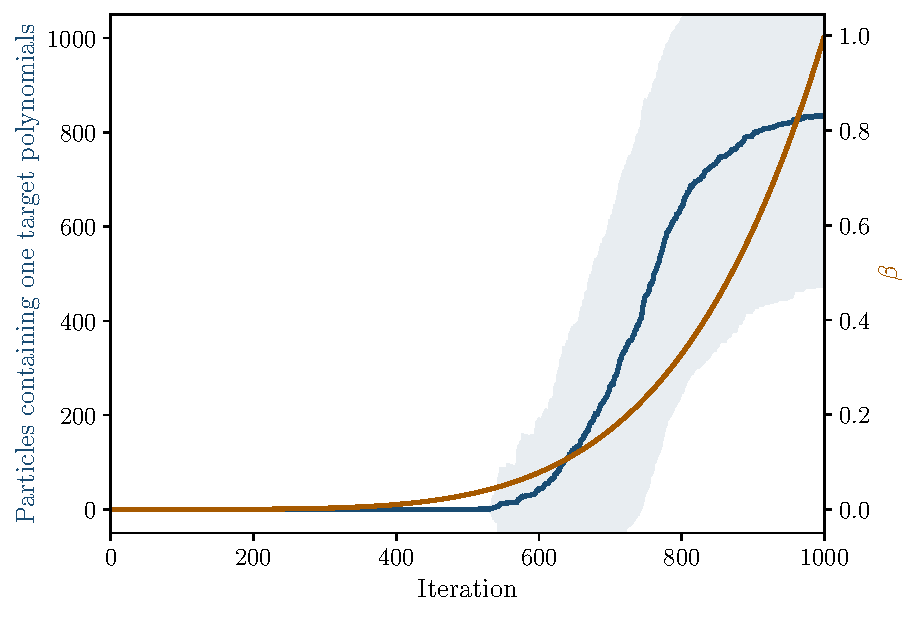
\includegraphics[scale=0.75]{Figures/Count_beta_history_2025_05_18_at_06_28_32.pdf}};
	  		\draw ($(fig1.north west) + (0,0)$) node {\small (a)};
	  		\draw (0,-8) node (fig2) {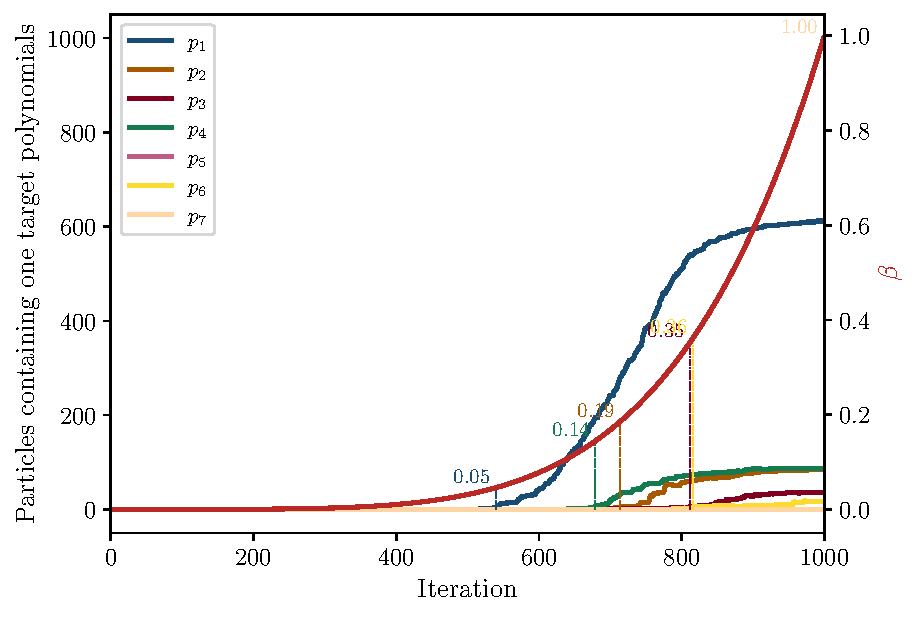
\includegraphics[scale=0.75]{Figures/Count_beta_history_2025_05_18_at_06_28_32_detailed.pdf}};
	  		\draw ($(fig2.north west) + (0,0)$) node {\small (b)};
	  	\end{tikzpicture}
	  	\caption{(a) Evolution of the mean numbers of particles reproducing a target polynomials and its $1\sigma$ deviation for the parameters~\eqref{eq:sample10000beta5}. (b) Evolution of the mean numbers of particles reproducing each targets polynomial. The vertical lines indicate when there are an average 5 particles reproducing a given polynomial, and the value of $\beta$ at that moment.}
	  	\label{fig:sample10000beta5}
	  \end{figure}

	  \item For 100 runs with parameters
		\begin{equation} \label{eq:sample10000beta3}
			\begin{gathered}
				\texttt{max degree} = 4, \quad \texttt{max num monomials} = 6, \quad n_{\rm iter} = 1000, \quad n_{\rm particles} = 1000, \\
				\texttt{sample size} = 10000, \quad {\rm reg} = 10^{3}, \quad \beta = 10^{-10} + \left(\frac{i}{n_{\rm iter}}\right)^{3}, \quad \sigma = 0.1, \\
				p_{\rm add} = 0, \quad p_{\rm remove} = 0, \quad p_{\rm modify} = 0.5, \quad p_{\rm multiply} = 0.25, \quad p_{\rm divide} = 0.25,
			\end{gathered}
		\end{equation}
		the polynomials are found at the following frequencies
	  \begin{equation}
	  	\begin{tabular}{l|cccccccc}
	  		& $p_{1}$ & $p_{2}$ & $p_{3}$ & $p_{4}$ & $p_{5}$ & $p_{6}$ & $p_{7}$ & $\varnothing$ \\\hline\hline
	  		Frequency & 76\% & 18\% & 10\% & 6\% & 4\% & 1\% & 2\% & 6\%
	  	\end{tabular}
	  \end{equation}
	  The dynamics of the appearance of the target polynomials is plotted in fig.~\ref{fig:sample10000beta3}.

	  Averaged number of particles reproducing a target in a successful run: $973 \pm 103$

	  Mean loss with regularisation for particles reproducing a target: $310 \pm 115$

	  Mean loss without regularisation for particles reproducing a target: $58 \pm 40$

	  \begin{figure}[h!]
	  	\centering
	  	\begin{tikzpicture}
	  		\draw (0,0) node (fig1) {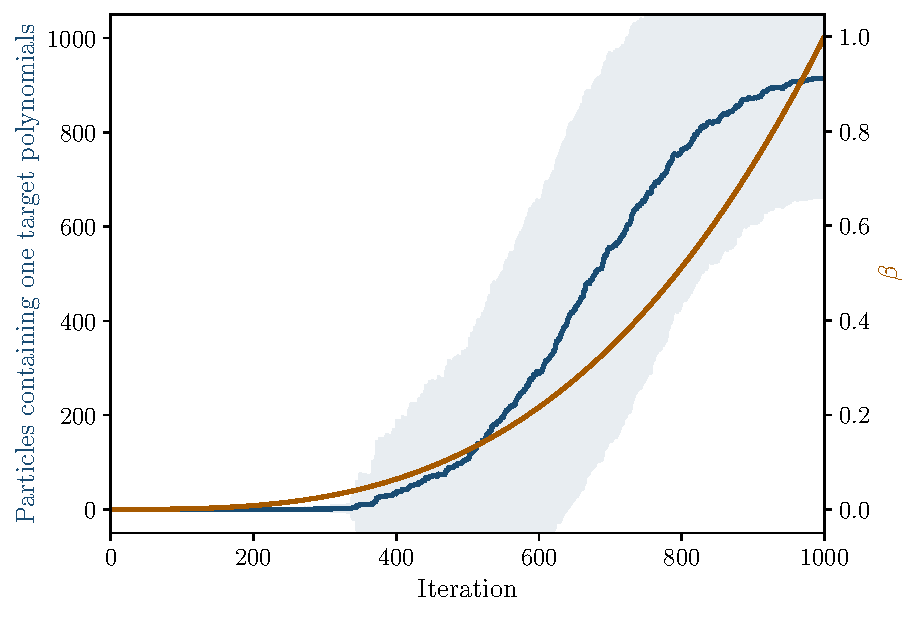
\includegraphics[scale=0.75]{Figures/Count_beta_history_2025_05_19_at_06_01_21.pdf}};
	  		\draw ($(fig1.north west) + (0,0)$) node {\small (a)};
	  		\draw (0,-8) node (fig2) {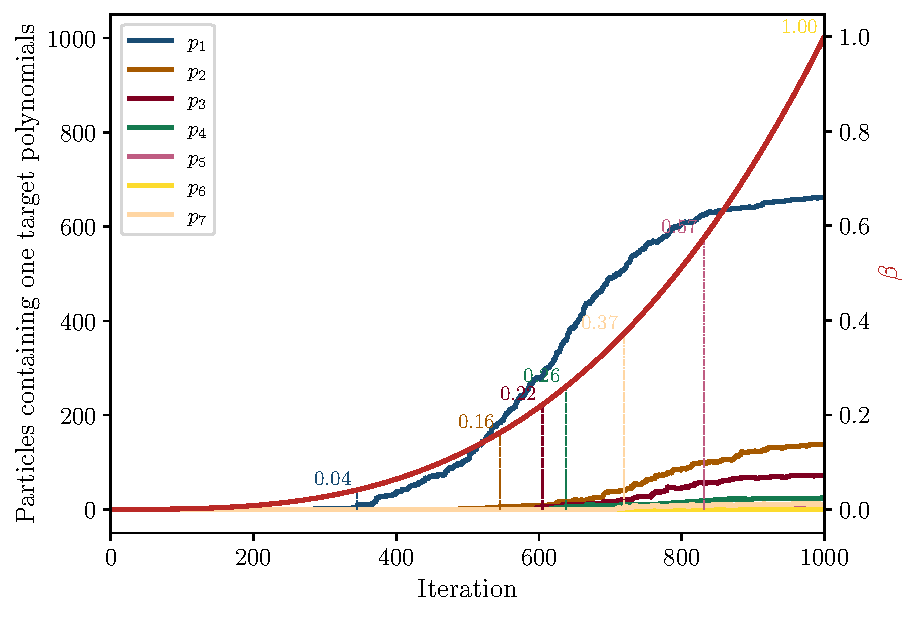
\includegraphics[scale=0.75]{Figures/Count_beta_history_2025_05_19_at_06_01_21_detailed.pdf}};
	  		\draw ($(fig2.north west) + (0,0)$) node {\small (b)};
	  	\end{tikzpicture}
	  	\caption{Evolution of the mean numbers of particles reproducing a target polynomials and its $1\sigma$ deviation for the parameters~\eqref{eq:sample10000beta3}. (b) Evolution of the mean numbers of particles reproducing each targets polynomial. The vertical lines indicate when there are an average 5 particles reproducing a given polynomial, and the value of $\beta$ at that moment.}
	  	\label{fig:sample10000beta3}
	  \end{figure}

	  \item For 100 runs with parameters
		\begin{equation} \label{eq:sample1000}
			\begin{gathered}
				\texttt{max degree} = 4, \quad \texttt{max num monomials} = 6, \quad n_{\rm iter} = 1000, \quad n_{\rm particles} = 1000, \\
				\texttt{sample size} = 1000, \quad {\rm reg} = 10^{3}, \quad \beta = 10^{-10} + \left(\frac{i}{n_{\rm iter}}\right)^{5}, \quad \sigma = 0.1, \\
				p_{\rm add} = 0, \quad p_{\rm remove} = 0, \quad p_{\rm modify} = 0.5, \quad p_{\rm multiply} = 0.25, \quad p_{\rm divide} = 0.25,
			\end{gathered}
		\end{equation}
		the polynomials are found at the following frequencies
	  \begin{equation}
	  	\begin{tabular}{l|cccccccc}
	  		& $p_{1}$ & $p_{2}$ & $p_{3}$ & $p_{4}$ & $p_{5}$ & $p_{6}$ & $p_{7}$ & $\varnothing$ \\\hline\hline
	  		Frequency & 72\% & 27\% & 3\% & 19\% & 2\% & 0\% & 0\% & 12\%
	  	\end{tabular}
	  \end{equation}
	  The dynamics of the appearance of the target polynomials is plotted in fig.~\ref{fig:sample1000}.

	  Averaged number of particles reproducing a target in a successful run: $401 \pm 389$

	  Mean loss with regularisation for particles reproducing a target: $406 \pm 193$ \ce{Needs to be renormalized by the sample size.}

	  Mean loss without regularisation for particles reproducing a target: $272 \pm 192$ \ce{Needs to be renormalized by the sample size.}

	  \begin{figure}[h!]
	  	\centering
	  	\begin{tikzpicture}
	  		\draw (0,0) node (fig1) {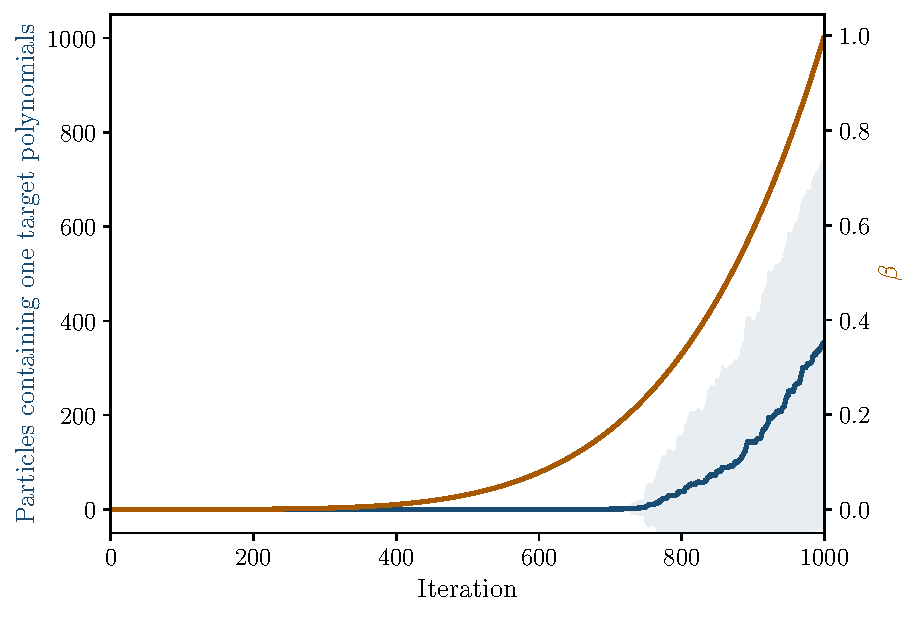
\includegraphics[scale=0.75]{Figures/Count_beta_history_2025_05_20_at_08_01_44.pdf}};
	  		\draw ($(fig1.north west) + (0,0)$) node {\small (a)};
	  		\draw (0,-8) node (fig2) {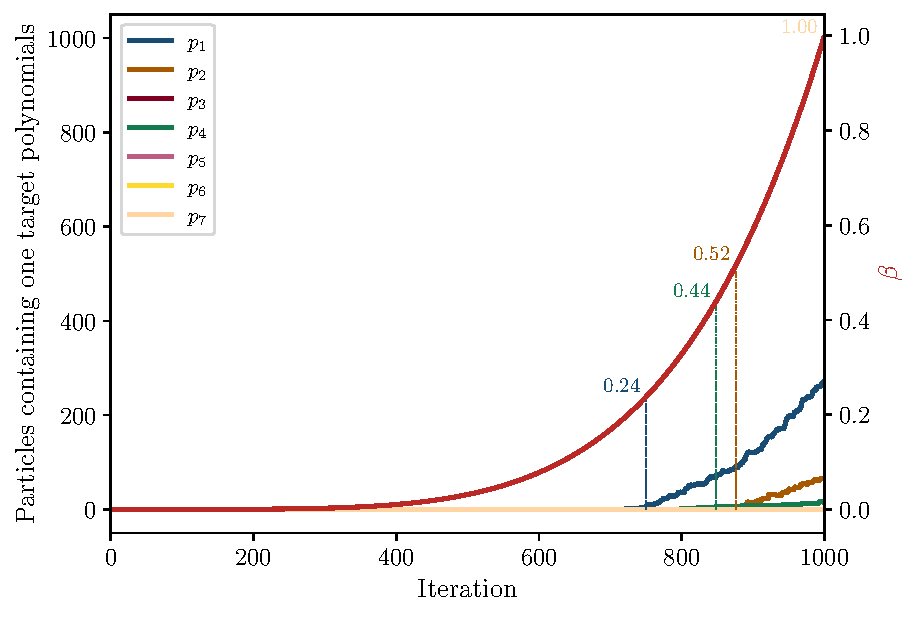
\includegraphics[scale=0.75]{Figures/Count_beta_history_2025_05_20_at_08_01_44_detailed.pdf}};
	  		\draw ($(fig2.north west) + (0,0)$) node {\small (b)};
	  	\end{tikzpicture}
	  	\caption{Evolution of the mean numbers of particles reproducing a target polynomials and its $1\sigma$ deviation for the parameters~\eqref{eq:sample1000}. (b) Evolution of the mean numbers of particles reproducing each targets polynomial. The vertical lines indicate when there are an average 5 particles reproducing a given polynomial, and the value of $\beta$ at that moment.}
	  	\label{fig:sample1000}
	  \end{figure}
  \end{enumerate}
	

  \ce{Draw histograms of the polynomials distribution to discuss runs with multiple outputs?}

\section{Supergravity solutions}
\begin{itemize}[label=\textbullet]
	\item For each couple of candidate polynomials, we get the same expression for the solution, and it indeed defines a unique vacuum of the 3d SUGRA.
	\item Discussion of the vacuum: gauge group, Zham. metric, change of variables, 3d spectrum (and stability), spin 2 spectrum on $S^{3}$, one parameter seems to be a gauge parameter, uplift?
\end{itemize}

For every couples $(p_{i},p_{j})$ of polynomials in eq.~\eqref{eq:pols}, the system
\begin{equation}
	\begin{cases}
		p_{i} = 0, \\
		p_{j} = 0,
	\end{cases}
\end{equation}
gives the same solution \ce{That's not true! For example, $x_{1}=x_{2}=0$ solves all polynomials but is not a sugra solution. Mention tests on the sugra?}
\begin{equation}
	\begin{cases}
		\displaystyle x_{1} = \frac{x_{2}}{\sqrt{2}}\,\frac{e^{x_{8}/2}}{e^{x_{8}}-1}\,\Big(-x_{5}\,e^{x_{8}/2} + \sqrt{2-4\,e^{x_{8}}+e^{2x_{8}}\big(2+x_{10}^{2}\big)}\Big),\\[8pt]
		\displaystyle x_{4} = \frac{e^{-x_{8}/2}}{\sqrt{2}}\,\sqrt{2-4\,e^{x_{8}}+e^{2x_{8}}\big(2+x_{10}^{2}\big)}.
	\end{cases}
\end{equation}
We checked that this defines a 3-parameter solution of three-dimensional half-maximal supergravity. Equivalently:
\begin{equation}
	\begin{cases}
		\displaystyle \tilde{x}_{8} = \frac{x_{1}^{2}+x_{2}^{2}}{x_{2}^{2} + \big(x_{1}-x_{2}x_{4}\big)^{2}},\\[10pt]
		\displaystyle x_{10} = \sqrt{2}\,x_{4}\,\frac{x_{2}^{2} - x_{1}^{2}+x_{1}x_{2}x_{4}}{x_{1}^{2}+x_{2}^{2}}.
	\end{cases}
\end{equation}
The solution preserves a ${\rm U}(1)\times{\rm U}(1)$ gauged symmetry.

\paragraph{Moduli space}
The $(x_{1},x_{2},x_{4})$ moduli space is most nicely parametrised using the change of coordinates
\begin{equation}
	x_{1} = r\cos(\theta)\cos(\Phi), \quad x_{2} = r\cos(\theta)\sin(\Phi) \quad {\rm and} \quad x_{4} = r\sin(\theta),
\end{equation}
for which the Zamolodchikov metric reads
\begin{equation}
	\d^{2}s_{\rm Zam.} = -\,\d r^{2} - r^{2}\,\bigg(\d \theta^{2} - r\cos(\theta)\,\d \theta\d\Phi + \sin(\theta)\,\d r\d\Phi + \frac{1}{2}\,\big(3+r^{2}-\cos(2\theta)\big)\,\d\Phi^{2} \bigg).
\end{equation}
\ce{Tests other change of variables? Test choices of variables other than $(x_{1},x_{2},x_{4})$?}

\paragraph{Bosonic spectrum}
Vector fields:
\begin{equation}
 \begin{aligned}	
	m_{\sst{(1)}}\ell_{\rm AdS}:\quad &
	0\ [2],	\quad
	-2\ [5],	\quad
	2\ [1],	\\[5pt]
	&	-1\pm\sqrt{\left(1+r^2\right)^2-2\,r^2\,\cos(2\theta)}\ [2+2],	\\[5pt]
	&	1\pm\sqrt{1+4\,r^2+r^{4}}\ [2+2].
 \end{aligned}
\end{equation}
The integers between square brackets indicate the multiplicity of each eigenvalue. The spectrum includes two massless vectors corresponding to the unbroken ${\rm U}(1)\times {\rm U}(1)$ gauge symmetry, although in three dimensions they are non-propagating.


Scalars:
\begin{equation}
 \begin{aligned}	
	\left(m_{\sst{(0)}}\ell_{\rm AdS}\right)^2:\quad&
	0\ [5],	\quad
	8\ [1],	\quad
	r^{2}\,\left(4+r^2\right)\ [8],	\\[5pt]
	&	2r\,\Big(3\,r+r^{3}\pm(2+r^{2})\,\sqrt{2+r^2-2\,\cos(2\theta)}-r\cos(2\theta)\Big)\ [2+2].
 \end{aligned}
\end{equation}

Gravitini:
\begin{equation}
	m_{{(\nicefrac32)}}\ell_{\rm AdS}:\quad 
	\quad \dfrac1{2}\bigg[1\pm\sqrt{4+2\,r^{2}+r^{4}-2r^{2}\cos(2\theta)}\bigg]\ [4+4],
\end{equation}
no SUSY enhancements other than $r=0$.

No dependence on $\Phi$.

\section{Conclusion}
\begin{itemize}[label=\textbullet]
	\item Conclusion: good prospects of improvement to be able to access higher dimensional cases. Classify flat directions.
	\item Appendix with some details on the code?
\end{itemize}


\bibliography{references}


\end{document}